\subsection{N型分次余代数的性质}

命题5. (i) 设 E 是一个具有余单位 \(\gamma\) 的分次余代数；则 \(\gamma\) 是次数为 0 的齐次线性形式。

\begin{enumerate}
\def\labelenumi{(\roman{enumi})}
\setcounter{enumi}{1}
\tightlist
\item
  进一步假设存在一个元素 \(e \in \mathbf{E}\) ，使得 \(\mathbf{E}_0 = \mathbf{A}e\) 且 \(\gamma(e) = 1\) 。那么 \(\mathbf{E}_{\gamma}\) （即 \(\gamma\) 的核）等于 \(\mathbf{E}_{+} = \sum_{n \geqslant 1} \mathbf{E}_n, c(e) = e \otimes e\) 和
\end{enumerate}

\[
c (x) \equiv x \otimes e + e \otimes x (\mathrm{mod.} \mathrm{E} _ {+} \otimes \mathrm{E} _ {+})\tag{19}
\]

对所有 \(x \in \mathbf{E}_{+}\) 。

\begin{enumerate}
\def\labelenumi{(\roman{enumi})}
\tightlist
\item
  只需验证 \(\gamma(x) = 0\) （对 \(x \in \mathbf{E}_n\) ，对所有 \(n \geqslant 1\) ）。由于 \(c\) 是次数为 0 的分次同态，
\end{enumerate}

\[
c (x) = \sum_ {0 \leqslant j \leqslant n} \left(\sum_ {i} y _ {i j} \otimes z _ {i, n - j}\right)\tag{20}
\]

其中，对所有 \(j\) （满足 \(0 \leqslant j \leqslant n\) ）， \(y_{ij}\) 和 \(z_{ij}\) 在 \(\mathbf{E}_j\) 中；应用（16）（第2号），我们得到

\[
x = \sum_ {0 \leqslant j \leqslant n} \left(\sum_ {i} \gamma (y _ {i j}) z _ {i, n - j}\right) = \sum_ {0 \leqslant j \leqslant n} \left(\sum_ {i} \gamma (z _ {i, n - j}) y _ {i j}\right),
\]

因此，比较两边次数为0和次数为n的分量，可得

\[
x = \sum_ {i} \gamma (y _ {i 0}) z _ {i n} = \sum_ {i} \gamma (z _ {i 0}) y _ {i n}
\]

\[
0 = \sum_ {i} \gamma (y _ {i n}) z _ {i 0} = \sum_ {i} \gamma (z _ {i n}) y _ {i 0}
\]

从而 \(\gamma(x) = \sum_{i} \gamma(y_{in})\gamma(z_{i0}) = \gamma(0) = 0\) 。

\begin{enumerate}
\def\labelenumi{(\roman{enumi})}
\setcounter{enumi}{1}
\tightlist
\item
  由于 \(\operatorname{Ker}(\gamma)\) 和 \(\mathbf{E}_{+}\) 都是 \(Ae = E_0\) 的补子模，且由（i）有 \(\mathbf{E}_{+} \subset \operatorname{Ker}(\gamma)\) ，故 \(\mathbf{E}_{+} = \operatorname{Ker}(\gamma)\) (II，§1，第8号，注记1)；其余断言由第2号命题4推出。
\end{enumerate}

命题6. 设E为A上的分次余代数。为使对每个交换A-代数B（具有平凡分次），型为Z的分次A-代数Homgr \(_{A}\) (E, B)（第2号）是反交换的（§4，第9号，定义7），其充分必要条件为，若 \(\sigma_{g}\) 表示 A-模 E \(\otimes_{A} E\) 的自同构，使得

\[
\sigma_ {g} (x _ {p} \otimes x _ {q}) = (- 1) ^ {p q} x _ {q} \otimes x _ {p}
\]

对 \(x_{p} \in \mathbf{E}_{p}, x_{q} \in \mathbf{E}_{q}\) （其中 \(p\) 和 \(q\) 是 \(\mathbf{N}\) 中的任意元素），该图表

\begin{enumerate}
\def\labelenumi{(\arabic{enumi})}
\setcounter{enumi}{20}
\tightlist
\item
\end{enumerate}

\pandocbounded{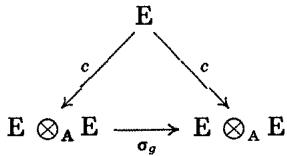
\includegraphics[keepaspectratio]{images/part004_b841500b.jpg}}

是交换的。

证明与第2号的命题2的证明类似。

当分次余代数 E 满足命题6的条件时，称其为余反交换的。

例。由第1号公式 (8) 直接可得，对每个 A-模 M，分次余代数 \(\bigwedge(M)\) 是余反交换的。

